% Created 2017-10-20 Fri 11:03
% Intended LaTeX compiler: pdflatex
\documentclass[10pt,oneside,x11names]{article}
\usepackage[utf8]{inputenc}
\usepackage[T1]{fontenc}
\usepackage{graphicx}
\usepackage{grffile}
\usepackage{longtable}
\usepackage{wrapfig}
\usepackage{rotating}
\usepackage[normalem]{ulem}
\usepackage{amsmath}
\usepackage{textcomp}
\usepackage{amssymb}
\usepackage{capt-of}
\usepackage{hyperref}
\usepackage{geometry}
\usepackage{palatino}
\usepackage{siunitx}
\usepackage{braket}
\usepackage[euler-digits,euler-hat-accent]{eulervm}
\author{Brian Beckman, Uri Ran}
\date{\textit{<2015-11-23 Mon>}}
\title{Uri's SM in Lisp: Version 0.0.4}
\hypersetup{
 pdfauthor={Brian Beckman, Uri Ran},
 pdftitle={Uri's SM in Lisp: Version 0.0.4},
 pdfkeywords={},
 pdfsubject={},
 pdfcreator={Emacs 24.3.1 (Org mode 8.0.7)},
 pdflang={English}}
\begin{document}

\maketitle
\setcounter{tocdepth}{2}
\tableofcontents


\section{Preliminaries}
\label{sec:org864d3e0}

\begin{verbatim}
Emacs version: GNU Emacs 25.3.1 (x86_64-apple-darwin13.4.0, NS appkit-1265.21 Version 10.9.5 (Build 13F1911))
 of 2017-09-12
org version: 9.0.9
\end{verbatim}

This is version 0.0.4 of Uri Ran's State-Machine demo.

\subsection{How to Use this Document}
\label{sec:org546c49d}

This is a literate program. Code and documentation cohabit a single
``org-mode'' file called \texttt{sm3.org}. Typeset the document by running the emacs
command \texttt{org-latex-export-to-pdf}. If you're a VIM user, use
\emph{Spacemacs}\footnote{\url{http://spacemacs.org}}, a near-perfect emulation of VIM in emacs. See the
section ``Running Code'' for instructions on running the code in this document.

\subsection{Setup}
\label{sec:org58a2284}

\section{Vertex Struct}
\label{sec:org9c9f410}

A \emph{vertex} or ``state'' in the state-machine diagram has an \emph{entry action}, a
\emph{do-action}, an \emph{exit-action}, and an \emph{event table}.  We prefer the word
``vertex'' to reduce ambiguity and overloading of the word ``state.''

Consider a unique variable or \emph{token} called \texttt{*current-vertex*}. The value of
this token represents the vertex that the state machine \emph{inhabits}. The state
machine may inhabit exactly one vertex at any time. Visualize the dynamics of
the machine as a sequence of indivisible, atomic steps in which the token
either stays within the current vertex or moves from one vertex to another in
response to \emph{events} or \emph{inputs}. Events or inputs are denoted by \emph{symbols}
drawn from a finite \emph{alphabet}, one at a time.

Entry actions run whenever the \texttt{*current-vertex*} token enters a vertex.
Exit actions run when the \texttt{*current-vertex*} token leaves a vertex.

Do-actions concern \emph{polling}, not further discussed here. Although we define
do-actions here, we don't use them; they're a placeholder in this version.

An \emph{event table} is an associative lookup table from event symbols to a list
of triples. Each triple has a Boolean-valued \emph{guard function}, a
\emph{transition-action} function, and a new vertex. The engine will \texttt{funcall} the
guards in the list, in the order they're presentated, and accept the first
triple whose guard returns \texttt{t}, which means \emph{true} in Lisp. ``Accepting the
triple'' means running the \emph{transition action} and moving the token to the new
vertex if the new vertex is non-nil (TODO: what if the new vertex is \emph{nil}?).
The exit action of the old vertex runs and then the entry action of the new
vertex runs. If no guards return \texttt{t}, the engine logs a trace message and does
nothing.

The following lisp code defines the vertex struct.

\begin{verbatim}
(defstruct vertex-t name entry-ac do-ac exit-ac evt-tbl)
\end{verbatim}

\texttt{defstruct} gives us basic constructors and accessors, and that's all we need
for this demonstration. Should we need more in the future, we can consider
Lisp's \texttt{defclass}.

As a side-effect of calling \texttt{defstruct}, Lisp defines the following functions
in our environment

\begin{itemize}
\item \texttt{(make-vertex-t}
\begin{itemize}
\item \texttt{:name} \emph{<name your vertex>}
\item \texttt{:entry-ac} \emph{<put a function value here>}
\item \texttt{:do-ac} \emph{<put another function value>}
\item \texttt{:exit-ac} \emph{<put another function value>}
\item \texttt{:evt-tbl} \emph{<put an event table, here>} \texttt{)}
\item produces an instance of \texttt{vertex-t}; this is a \emph{constructor} function
\end{itemize}

\item \texttt{(vertex-t-name} \emph{<some instance of vertex-t>} \texttt{)} produces the name of the
vertex; this is like the dot notation in C / C++, \emph{i.e.}, like \texttt{someInstance.name}

\item \texttt{(vertex-t-entry-ac} \emph{<some instance of vertex-t>} \texttt{)} produces the
entry-action function value of the vertex; also like dot, just for a
different instance variable

\item \texttt{(vertex-t-do-ac} \emph{<some instance of vertex-t>} \texttt{)} produces the
do-action function value of the vertex; ditto

\item \texttt{(vertex-t-exit-ac} \emph{<some instance of vertex-t>} \texttt{)} produces the
exit-action function value of the vertex; etc.

It's possible to mutate the \emph{instance variables} of a \texttt{defstruct}, but we
don't need to do this here.
\end{itemize}

\section{Utilities}
\label{sec:orgb9d214a}
\subsection{Boolean fair coin}
\label{sec:orgdbe2c35}

For fuzz testing.

\begin{verbatim}
(defun coin () (= 0 (random 2)))
\end{verbatim}

\subsection{Take \& Drop}
\label{sec:org2458542}

\begin{verbatim}
(defun take (seq n)
  "(take seq n) gives the first n elements of the seq. (take seq -n) gives the
  last n elements of the seq. This works on strings as well."
  (check-type seq sequence)
  (check-type n integer)
  (let ((l (length seq)))
    (cond ((>= n 0) (subseq seq 0 (min n l)))
          ((<  n 0) (subseq seq (max 0 (+ n l)) l))
          ((=  n 0) (subseq seq 0 0)))))

(defun drop (seq n)
  "(drop seq n) gives the seq with the first n elements removed. (drop seq -n)
  gives the seq with the last n elements removed. This works on strings as
  well."
  (let ((l (length seq)))
    (check-type seq sequence)
    (check-type n integer)
    (cond ((>= n 0) (subseq seq (min n l) l))
          ((<  n 0) (subseq seq 0 (max 0 (+ n l))))
          ((=  n 0)  seq))))

(defun str-last (str)
  "(str-last non-empty-string) produces the last character in a non-empty
  string."
  (check-type str string)
  (let ((l (length str)))
    (assert (> l 0))
    (subseq str (- l 1) l)))
\end{verbatim}

\subsection{Drawing to DOT}
\label{sec:org13aedc1}

Borrowed from ``Land of Lisp'' by Conrad Barski, M.D.

\subsubsection{{\bfseries\sffamily TODO} Robustify}
\label{sec:org5d01729}

a-la \url{http://tinyurl.com/y63ugo} and \url{http://tinyurl.com/j23lakq}


\begin{verbatim}
(defparameter *max-label-length* 30)
\end{verbatim}

\begin{verbatim}
(defun dot-name (exp)
  (substitute-if #\_ (complement #'alphanumericp) (prin1-to-string exp)))

(defun dot-label (exp)
  (if exp
      (let ((s (write-to-string exp :pretty nil)))
        (if (> (length s) *max-label-length*)
            (concatenate 'string (subseq s 0 (- *max-label-length* 3)) "...")
            s))
      ""))

(defun nodes->dot (nodes)
  (mapc (lambda (node)
          (fresh-line)
          (princ (dot-name (car node)))
          (princ "[label=\"")
          (princ (dot-label node))
          (princ "\"];"))
        nodes))

(defun edges->dot (edges)
  (mapc (lambda (node)
          (mapc (lambda (edge)
                  (fresh-line)
                  (princ (dot-name (car node)))
                  (princ "->")
                  (princ (dot-name (car edge)))
                  (princ "[label=\"")
                  (princ (dot-label (cdr edge)))
                  (princ "\"];"))
                (cdr node)))
        edges))

(defun dgraph->dot (nodes edges)
  (princ "digraph{")
  (nodes->dot nodes)
  (edges->dot edges)
  (princ "}"))

(defun uedges->dot (edges)
  (maplist (lambda (lst)
             (mapc (lambda (edge)
                     (unless (assoc (car edge) (cdr lst))
                       (fresh-line)
                       (princ (dot-name (caar lst)))
                       (princ "--")
                       (princ (dot-name (car edge)))
                       (princ "[label=\"")
                       (princ (dot-label (cdr edge)))
                       (princ "\"];")))
                   (cdar lst)))
           edges))

(defun ugraph->dot (nodes edges)
  (princ "graph{")
  (nodes->dot nodes)
  (uedges->dot edges)
  (princ "}"))

(defun dot->png (fname thunk)
  (with-open-file (*standard-output* (concatenate 'string fname ".dot") :direction :output :if-exists :supersede)
    (funcall thunk))
  ;; (ext:shell (concatenate 'string "dot -Tpng -O " fname ".dot"))
  )

(defun dgraph->png (fname nodes edges)
  (dot->png fname
            (lambda ()
              (dgraph->dot nodes edges))))

(defun ugraph->png (fname nodes edges)
  (dot->png fname
            (lambda ()
              (ugraph->dot nodes edges))))
\end{verbatim}

\section{Action and Guard Functions}
\label{sec:org1497fc9}

\subsection{Actions}
\label{sec:orgb3a22ab}

\subsubsection{{\bfseries\sffamily TODO} Parameters or return values for actions?}
\label{sec:org7679c94}

\subsubsection{{\bfseries\sffamily TODO} Contexts for actions and guards}
\label{sec:org6ab7017}

\subsubsection{Vertex Actions}
\label{sec:orge65f317}

For entry, polling (undefined) and exit, respectively.

Our actions just print to standard output because this is just a demo.  They
might do arbitrary side effects.

\begin{verbatim}
(defun vertex-1-entry () (print "vertex 1 entry"))
(defun vertex-2-entry () (print "vertex 2 entry"))
(defun vertex-3-entry () (print "vertex 3 entry"))
(defun vertex-4-entry () (print "vertex 4 entry"))

(defun vertex-1-do    () (print "vertex 1 do"))
(defun vertex-2-do    () (print "vertex 2 do"))
(defun vertex-3-do    () (print "vertex 3 do"))
(defun vertex-4-do    () (print "vertex 4 do"))

(defun vertex-1-exit  () (print "vertex 1 exit"))
(defun vertex-2-exit  () (print "vertex 2 exit"))
(defun vertex-3-exit  () (print "vertex 3 exit"))
(defun vertex-4-exit  () (print "vertex 4 exit"))
\end{verbatim}

\subsubsection{Edge Actions}
\label{sec:org98dbcee}

When the engine takes a transition, moving the token from one vertex to
another, it runs these functions.

\begin{verbatim}
(defun act-a () (print "action a" ))
(defun act-b () (print "action b" ))
(defun act-c () (print "action c" ))
(defun act-d () (print "action d" ))
(defun act-na() (print "action na"))
\end{verbatim}

\subsection{Guards (Boolean-Valued)}
\label{sec:orge6bc995}

\begin{verbatim}
(defun guard-x     () (coin) )
(defun guard-y     () (coin) )
(defun guard-z     () (coin) )
(defun guard-true  () t      )
(defun guard-false () nil    )
(defun guard-na    () t      )
\end{verbatim}

\section{The Diagram}
\label{sec:org26671ce}

If \texttt{nym} is \(\texttt{"foo"}\), we want functions \texttt{foo-entry}, \texttt{foo-do}, and
\texttt{foo-exit} automatically assigned.  The following macro expands into the
boilerplate necessary for creating instances of \texttt{vertex-t}. These instances
are stored in global \emph{special variables} demarcated with asterisks, for
example, \texttt{*vertex-1*}. Special variables are basically global variables, but
there are some subtleties that don't concern us here.\footnote{\url{http://www.flownet.com/ron/specials.pdf}}

The macro works by defining some strings for the identifiers based off the
\texttt{nym}, converting them to symbols, and writing out new code that defines,
via \texttt{defvar}, a global variable that refers to an instance of \texttt{vertex-t}
with \emph{entry}, \emph{do}, and \emph{exit} actions defined according to the naming
convention in the paragraph above.

\subsection{How to Define a Vertex}
\label{sec:orgd416e92}

\begin{verbatim}
(defparameter *vertices* nil)
(defmacro defvertex (nym evt-tbl)
  (let* ((dynvar (format nil "*~A*"     nym))
         (entry  (format nil "~A-entry" nym))
         (doo    (format nil "~A-do"    nym))
         (exit   (format nil "~A-exit"  nym))
         (vtxsym (with-input-from-string (s dynvar) (read s))))
    `(progn
       (defparameter ,vtxsym
         (make-vertex-t
          :name     (format nil "~A" ,nym)
          :entry-ac (function ,(with-input-from-string (s entry) (read s)))
          :do-ac    (function ,(with-input-from-string (s doo  ) (read s)))
          :exit-ac  (function ,(with-input-from-string (s exit ) (read s)))
          :evt-tbl  ,evt-tbl))
       (push ,vtxsym *vertices*))))
\end{verbatim}

\subsection{Vertices in Our Diagram}
\label{sec:org0c5ac10}

Notice that the new vertices named in the event table are unevaluated symbols.
That's because we want to refer to them before they're defined. We know their
names at the time we write the table, but they don't always have values. This
is a good way to avoid forward referencing and resolution. Evaling the symbols
at transition time is preferable.

\begin{verbatim}
(defvertex "vertex-1"
    '((ev-2 (guard-true act-c  *vertex-3* ))
      (ev-3 (guard-x    act-na *vertex-1* ))  ))
(defvertex "vertex-2"
    '((ev-4 (guard-true act-na *vertex-1* ))
      (ev-6 (guard-x    act-c  *vertex-4* ))  ))
(defvertex "vertex-3"
    '((ev-1 (guard-x    act-na nil        )
            (guard-y    act-b  *vertex-1* )
            (guard-z    act-na *vertex-1* ))
      (ev-5 (guard-na   act-d  *vertex-4* ))  ))
(defvertex "vertex-4"
    '((ev-3 (guard-y    act-d  *vertex-2* ))
      (ev-6 (guard-x    act-c  *vertex-3* ))  ))
\end{verbatim}

\subsection{Drawing The Diagram}
\label{sec:org9316ce3}

\begin{verbatim}
(defparameter *wizard-nodes*
  '((v1 1)
    (v2 2)
    (v3 3)
    (v4 4)))

(defparameter *wizard-edges*
  '((v1 (v3 g-t  ev-2)
        (v1 g-x  ev-3))
    (v2 (v1 g-t  ev-4)
        (v4 g-x  ev-6))
    (v3 (v1 g-y  ev-1)
        (v1 g-z  ev-1)
        (v4 g-na ev-5))
    (v4 (v2 g-y  ev-3)
        (v3 g-x  ev-6))))
\end{verbatim}

\begin{verbatim}
(dgraph->png "wizard" *wizard-nodes* *wizard-edges*)
\end{verbatim}

\begin{verbatim}
dot -Tpng -O wizard.dot
\end{verbatim}
\begin{center}
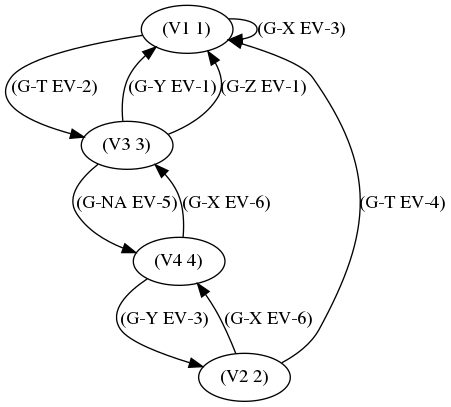
\includegraphics[width=.9\linewidth]{wizard.dot.png}
\end{center}

\subsection{Simulating Transitions in the Diagram}
\label{sec:org63d057b}

\subsubsection{The Vertex Token}
\label{sec:org24eb634}

At any time, the state-machine is ``in'' a vertex (or state). This means that
the value of \texttt{*current-vertex*} is the particular vertex instance. We call
\texttt{*current-vertex*} the \emph{vertex token}. Visualize a token on a gaming board
moving from one vertex to another.

\begin{verbatim}
(defparameter *current-vertex* *vertex-1*)
\end{verbatim}

\subsubsection{The Engine}
\label{sec:orgc5fe0b9}

\begin{enumerate}
\item Eval-First-Admissible-Triple
\label{sec:org6864f0e}

This function implements the token-moving strategy discussed above and
returns the current value of the token \texttt{*current-vertex*}, whether it's
changed or not.

When the new-vertex is \texttt{nil}, the \texttt{*current-vertex*} does not change and the
action functions do not run, even if the guard is true.

\begin{verbatim}
(defun eval-first-admissible-triple (triples)
  (cond (triples
         (let* ((triple     (first  triples))
                (guard      (first  triple))
                (action     (second triple))
                (new-vertex (eval (third  triple))))
           (if (and (funcall guard) new-vertex)
               (progn
                 (funcall (vertex-t-exit-ac *current-vertex*))
                 (funcall action)
                 (setf *current-vertex* new-vertex)
                 (funcall (vertex-t-entry-ac *current-vertex*)))
               (progn
                 (format t "~%~A: guard failed; trying next guard"
                         (vertex-t-name *current-vertex*))
                 (eval-first-admissible-triple (rest triples))))))
        (t (format t "~%~A: all guards failed; doing nothing"
                   (vertex-t-name *current-vertex*))))
  *current-vertex*)
\end{verbatim}

\item SM-Engine
\label{sec:org7114f59}

This takes an event symbol, does lookup in the diagram, and performs the
indicated transition.

\begin{verbatim}
(defun sm-engine (event-symbol)
  (let ((line (rest (assoc event-symbol
                           (vertex-t-evt-tbl *current-vertex*)))))
    (if line
        (eval-first-admissible-triple line)
        (progn
          (format t "~%~A: event ~W not found; doing nothing"
                  (vertex-t-name *current-vertex*)
                  event-symbol)
          *current-vertex*))))

\end{verbatim}
\end{enumerate}

\section{Running the Code}
\label{sec:org8f1d1df}

This document contains actual, live code. You can run the code in two ways:
inside org mode or by extracting (tangling) the code and running it at the
command line.

\subsection{Setting up Two Good Lisps}
\label{sec:org186676b}

Install SBCL (Steel Bank Common Lisp) for running this code in the editor or
a REPL, and ECL (Embeddable Common Lisp) for generating C code. On a mac,
this is trivial with homebrew:

\texttt{brew install sbcl}

\texttt{brew install ecl}

You will need SLIME in Emacs or Spacemacs to run the code in this file
directly. Just Google any of these things you don't recognize. I recommend
Spacemacs because it has high-fidelity VIM emulation.

To find out whether you have slime, type \texttt{M-x slime}. If you don't have it,
get it.

\subsection{Running Code Directly}
\label{sec:org1444305}

Once you have SLIME running in Emacs, type \texttt{M-x slime} to start the REPL,
then type \texttt{M-x org-babel-execute-buffer} to run all the code in this file. At
the very end of this file, you will see a few unit tests. Put the cursor in
that code block and type \texttt{C-c C-c} repeatedly to run the unit tests over and
over. The results will be slightly different each time because the guard
functions do coin flips. I have tried to arrange the unit tests so that the
last value always prints \texttt{t}, short for \texttt{true}.

\subsection{Extracting Code From This File}
\label{sec:orge32d444}

Type \texttt{M-x org-babel-tangle} and you should get a file named \texttt{sm.lisp}.

\subsection{Generating, Inspecting, Running C code}
\label{sec:org9bbf46b}

After extracting code, run ECL at the command prompt:
\begin{verbatim}
$ ecl -load make.lisp
\end{verbatim}
Watch all the pretty messages go by, then type
\begin{verbatim}
(quit)
\end{verbatim}
to leave the ECL REPL, then
\begin{verbatim}
$ ./sm
\end{verbatim}
to run the generated code. You should see exactly the same output as you
would get from the last section below.

\subsubsection{{\bfseries\sffamily TODO} Create Deeply Embedded C}
\label{sec:org2431914}

The generated code is in the files \texttt{sm.c}, \texttt{sm.h}, and \texttt{sm.data}.  The
generated code pretty much just calls the ECL runtime kernel. This is a
\emph{shallow embedding} of the lisp code in C.  A \emph{deep embedding} would write C
code that bypasses lisp-specific helpers and more directly express the model.
Bypassing a lisp runtime means that we can avoid exposure to garbage
collection and other potential hazards in the lisp implementation.

A good way to produce a deep embedding will be through macros.  The deeply
embedded code should be comparable to the code that Uri wrote by hand.

\subsection{Interactively}
\label{sec:org0ea24c6}

To run in an external REPL, paste the following code into the REPL (and remove
the quote, of course). Don't try to run this code from org-mode; it will
deadlock with SLIME as they contend over who has the terminal.

\begin{verbatim}
'(let ((ev 1024))
  (loop while (> ev 0) do
    (format t "~%Enter an event number > 0, 0 to quit: ")
    (setf ev (read))
    (format t "~%~A: searching for event ~A"
            (vertex-t-name *current-vertex*)
            (format nil "ev-~A" ev))
    (if (numberp ev)
        (progn
          (with-input-from-string (s (format nil "ev-~A" ev))
               (sm-engine (read s nil 0))))
        (format t "~%~A: failure: type-of ev wasn't a number, but a ~A"
                (vertex-t-name *current-vertex*)
                (type-of ev)))))

\end{verbatim}

\subsection{Unit Tests, Exhaustive Tests}
\label{sec:org1d8e79e}

Because the current guards are random, exhaustively testing them isn't as
trivial as enumeration.

Run the following unit test repeatedly; it can be a little different each
time, but the machine should always end up in vertex 3.

\begin{verbatim}
(print (equal *current-vertex* *vertex-1*))
(print (eq *current-vertex* *vertex-1*))
(print (eq (sm-engine 'ev-1) *vertex-1*))
(print (eq (sm-engine 'ev-4) *vertex-1*))
(print (eq (sm-engine 'bogus) *vertex-1*))
(print (eq (sm-engine 'ev-3) *vertex-1*))
(print (eq (sm-engine 'ev-2) *vertex-3*))
\end{verbatim}

\begin{verbatim}

T
T
vertex-1: event EV-1 not found; doing nothing
T
vertex-1: event EV-4 not found; doing nothing
T
vertex-1: event BOGUS not found; doing nothing
T
"vertex 1 exit"
"action na"
"vertex 1 entry"
T
"vertex 1 exit"
"action c"
"vertex 3 entry"
T
\end{verbatim}
Emacs 24.3.1 (Org mode 8.0.7)
\end{document}
